% Graphic for TeX using PGF
% Title: C:\Users\Nicolas Chicaiza\Dia\arbolProblemas.dia
% Creator: Dia v0.97.2
% CreationDate: Sun May 02 21:05:28 2021
% For: Nicolas Chicaiza
% \usepackage{tikz}
% The following commands are not supported in PSTricks at present
% We define them conditionally, so when they are implemented,
% this pgf file will use them.
\definecolor{titulo}{RGB}{41,56,69}
\begin{figure}[H]
	\centering
	\ifx\du\undefined
		\newlength{\du}
	\fi
	\setlength{\du}{15\unitlength}
	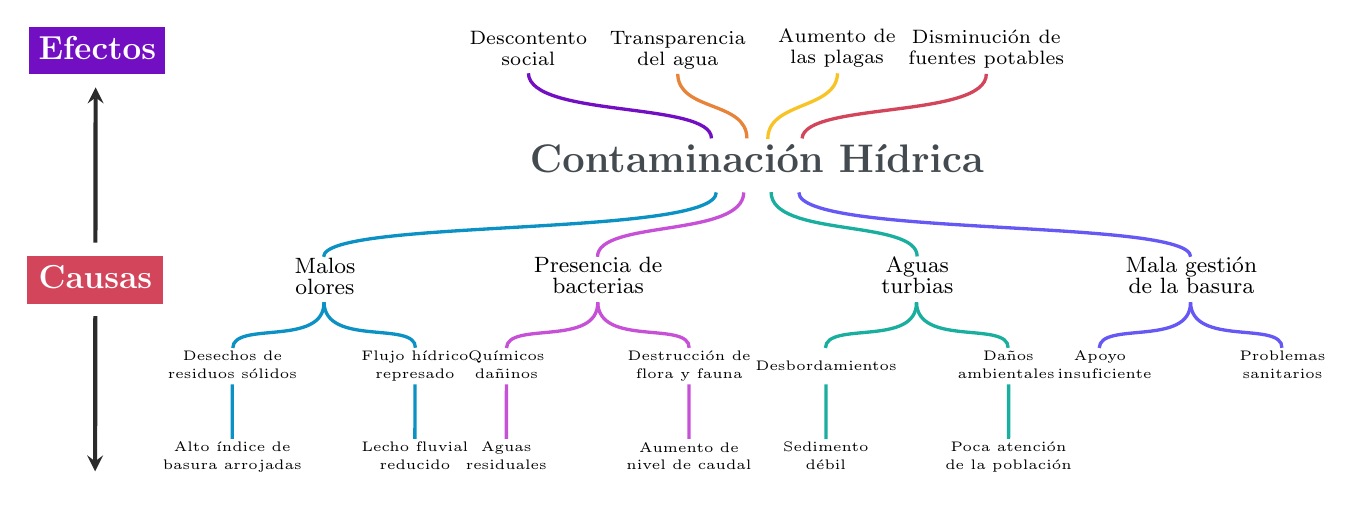
\begin{tikzpicture}[scale=1.1]
		\pgftransformxscale{1.000000}
		\pgftransformyscale{-1.000000}
		\definecolor{dialinecolor}{rgb}{0.000000, 0.000000, 0.000000}
		\pgfsetstrokecolor{dialinecolor}
		\pgfsetstrokeopacity{1.000000}
		\definecolor{diafillcolor}{rgb}{1.000000, 1.000000, 1.000000}
		\pgfsetfillcolor{diafillcolor}
		\pgfsetfillopacity{1.000000}
		% setfont left to latex
		\definecolor{dialinecolor}{rgb}{0.266667, 0.294118, 0.313726}
		\pgfsetstrokecolor{dialinecolor}
		\pgfsetstrokeopacity{1.000000}
		\definecolor{diafillcolor}{rgb}{0.266667, 0.294118, 0.313726}
		\pgfsetfillcolor{diafillcolor}
		\pgfsetfillopacity{1.000000}
		\node[anchor=base,inner sep=0pt, outer sep=0pt,color=dialinecolor] at (40.987812\du,21.163697\du){\Large{\textbf{Contaminación Hídrica}}};
		\pgfsetlinewidth{0.080000\du}
		\pgfsetdash{}{0pt}
		\pgfsetmiterjoin
		\pgfsetbuttcap
		{
			\definecolor{diafillcolor}{rgb}{0.450980, 0.058824, 0.764706}
			\pgfsetfillcolor{diafillcolor}
			\pgfsetfillopacity{1.000000}
			% was here!!!
			\definecolor{dialinecolor}{rgb}{0.450980, 0.058824, 0.764706}
			\pgfsetstrokecolor{dialinecolor}
			\pgfsetstrokeopacity{1.000000}
			\pgfpathmoveto{\pgfpoint{39.992568\du}{20.416076\du}}
			\pgfpathcurveto{\pgfpoint{40.005295\du}{19.601535\du}}{\pgfpoint{36.021678\du}{19.970624\du}}{\pgfpoint{35.983496\du}{18.990629\du}}
			\pgfusepath{stroke}
		}
		\pgfsetlinewidth{0.080000\du}
		\pgfsetdash{}{0pt}
		\pgfsetmiterjoin
		\pgfsetbuttcap
		{
			\definecolor{diafillcolor}{rgb}{0.827451, 0.270588, 0.356863}
			\pgfsetfillcolor{diafillcolor}
			\pgfsetfillopacity{1.000000}
			% was here!!!
			\definecolor{dialinecolor}{rgb}{0.827451, 0.270588, 0.356863}
			\pgfsetstrokecolor{dialinecolor}
			\pgfsetstrokeopacity{1.000000}
			\pgfpathmoveto{\pgfpoint{41.978012\du}{20.416076\du}}
			\pgfpathcurveto{\pgfpoint{42.028921\du}{19.614262\du}}{\pgfpoint{46.025265\du}{19.983351\du}}{\pgfpoint{46.012538\du}{19.003356\du}}
			\pgfusepath{stroke}
		}
		\pgfsetlinewidth{0.080000\du}
		\pgfsetdash{}{0pt}
		\pgfsetmiterjoin
		\pgfsetbuttcap
		{
			\definecolor{diafillcolor}{rgb}{0.909804, 0.513726, 0.227451}
			\pgfsetfillcolor{diafillcolor}
			\pgfsetfillopacity{1.000000}
			% was here!!!
			\definecolor{dialinecolor}{rgb}{0.909804, 0.513726, 0.227451}
			\pgfsetstrokecolor{dialinecolor}
			\pgfsetstrokeopacity{1.000000}
			\pgfpathmoveto{\pgfpoint{40.768927\du}{20.416076\du}}
			\pgfpathcurveto{\pgfpoint{40.768927\du}{19.588808\du}}{\pgfpoint{39.267117\du}{19.830625\du}}{\pgfpoint{39.254389\du}{19.003356\du}}
			\pgfusepath{stroke}
		}
		% setfont left to latex
		\definecolor{dialinecolor}{rgb}{0.000000, 0.000000, 0.000000}
		\pgfsetstrokecolor{dialinecolor}
		\pgfsetstrokeopacity{1.000000}
		\definecolor{diafillcolor}{rgb}{0.000000, 0.000000, 0.000000}
		\pgfsetfillcolor{diafillcolor}
		\pgfsetfillopacity{1.000000}
		\node[anchor=base,inner sep=0pt, outer sep=0pt,color=dialinecolor] at (35.983496\du,18.351180\du){\scriptsize{Descontento}};
		% setfont left to latex
		\definecolor{dialinecolor}{rgb}{0.000000, 0.000000, 0.000000}
		\pgfsetstrokecolor{dialinecolor}
		\pgfsetstrokeopacity{1.000000}
		\definecolor{diafillcolor}{rgb}{0.000000, 0.000000, 0.000000}
		\pgfsetfillcolor{diafillcolor}
		\pgfsetfillopacity{1.000000}
		\node[anchor=base,inner sep=0pt, outer sep=0pt,color=dialinecolor] at (35.983496\du,18.809791\du){\scriptsize{social}};
		\pgfsetlinewidth{0.080000\du}
		\pgfsetdash{}{0pt}
		\pgfsetmiterjoin
		\pgfsetbuttcap
		{
			\definecolor{diafillcolor}{rgb}{0.968627, 0.764706, 0.145098}
			\pgfsetfillcolor{diafillcolor}
			\pgfsetfillopacity{1.000000}
			% was here!!!
			\definecolor{dialinecolor}{rgb}{0.968627, 0.764706, 0.145098}
			\pgfsetstrokecolor{dialinecolor}
			\pgfsetstrokeopacity{1.000000}
			\pgfpathmoveto{\pgfpoint{41.227107\du}{20.428803\du}}
			\pgfpathcurveto{\pgfpoint{41.227107\du}{19.601535\du}}{\pgfpoint{42.728918\du}{19.792443\du}}{\pgfpoint{42.754372\du}{18.990629\du}}
			\pgfusepath{stroke}
		}
		% setfont left to latex
		\definecolor{dialinecolor}{rgb}{0.000000, 0.000000, 0.000000}
		\pgfsetstrokecolor{dialinecolor}
		\pgfsetstrokeopacity{1.000000}
		\definecolor{diafillcolor}{rgb}{0.000000, 0.000000, 0.000000}
		\pgfsetfillcolor{diafillcolor}
		\pgfsetfillopacity{1.000000}
		\node[anchor=base,inner sep=0pt, outer sep=0pt,color=dialinecolor] at (39.254389\du,18.351180\du){\scriptsize{Transparencia}};
		% setfont left to latex
		\definecolor{dialinecolor}{rgb}{0.000000, 0.000000, 0.000000}
		\pgfsetstrokecolor{dialinecolor}
		\pgfsetstrokeopacity{1.000000}
		\definecolor{diafillcolor}{rgb}{0.000000, 0.000000, 0.000000}
		\pgfsetfillcolor{diafillcolor}
		\pgfsetfillopacity{1.000000}
		\node[anchor=base,inner sep=0pt, outer sep=0pt,color=dialinecolor] at (39.254389\du,18.809791\du){\scriptsize{del agua}};
		% setfont left to latex
		\definecolor{dialinecolor}{rgb}{0.000000, 0.000000, 0.000000}
		\pgfsetstrokecolor{dialinecolor}
		\pgfsetstrokeopacity{1.000000}
		\definecolor{diafillcolor}{rgb}{0.000000, 0.000000, 0.000000}
		\pgfsetfillcolor{diafillcolor}
		\pgfsetfillopacity{1.000000}
		\node[anchor=base,inner sep=0pt, outer sep=0pt,color=dialinecolor] at (42.741645\du,18.325726\du){\scriptsize{Aumento de}};
		% setfont left to latex
		\definecolor{dialinecolor}{rgb}{0.000000, 0.000000, 0.000000}
		\pgfsetstrokecolor{dialinecolor}
		\pgfsetstrokeopacity{1.000000}
		\definecolor{diafillcolor}{rgb}{0.000000, 0.000000, 0.000000}
		\pgfsetfillcolor{diafillcolor}
		\pgfsetfillopacity{1.000000}
		\node[anchor=base,inner sep=0pt, outer sep=0pt,color=dialinecolor] at (42.741645\du,18.784337\du){\scriptsize{las plagas}};
		% setfont left to latex
		\definecolor{dialinecolor}{rgb}{0.000000, 0.000000, 0.000000}
		\pgfsetstrokecolor{dialinecolor}
		\pgfsetstrokeopacity{1.000000}
		\definecolor{diafillcolor}{rgb}{0.000000, 0.000000, 0.000000}
		\pgfsetfillcolor{diafillcolor}
		\pgfsetfillopacity{1.000000}
		\node[anchor=base,inner sep=0pt, outer sep=0pt,color=dialinecolor] at (46.012538\du,18.338453\du){\scriptsize{Disminución de}};
		% setfont left to latex
		\definecolor{dialinecolor}{rgb}{0.000000, 0.000000, 0.000000}
		\pgfsetstrokecolor{dialinecolor}
		\pgfsetstrokeopacity{1.000000}
		\definecolor{diafillcolor}{rgb}{0.000000, 0.000000, 0.000000}
		\pgfsetfillcolor{diafillcolor}
		\pgfsetfillopacity{1.000000}
		\node[anchor=base,inner sep=0pt, outer sep=0pt,color=dialinecolor] at (46.012538\du,18.797064\du){\scriptsize{fuentes potables}};
		\pgfsetlinewidth{0.080000\du}
		\pgfsetdash{}{0pt}
		\pgfsetmiterjoin
		\pgfsetbuttcap
		{
			\definecolor{diafillcolor}{rgb}{0.776471, 0.317647, 0.843137}
			\pgfsetfillcolor{diafillcolor}
			\pgfsetfillopacity{1.000000}
			% was here!!!
			\definecolor{dialinecolor}{rgb}{0.776471, 0.317647, 0.843137}
			\pgfsetstrokecolor{dialinecolor}
			\pgfsetstrokeopacity{1.000000}
			\pgfpathmoveto{\pgfpoint{37.497450\du}{23.009990\du}}
			\pgfpathcurveto{\pgfpoint{37.499492\du}{22.192968\du}}{\pgfpoint{40.680937\du}{22.593243\du}}{\pgfpoint{40.701154\du}{21.599060\du}}
			\pgfusepath{stroke}
		}
		% setfont left to latex
		\definecolor{dialinecolor}{rgb}{0.000000, 0.000000, 0.000000}
		\pgfsetstrokecolor{dialinecolor}
		\pgfsetstrokeopacity{1.000000}
		\definecolor{diafillcolor}{rgb}{0.000000, 0.000000, 0.000000}
		\pgfsetfillcolor{diafillcolor}
		\pgfsetfillopacity{1.000000}
		\node[anchor=base,inner sep=0pt, outer sep=0pt,color=dialinecolor] at (37.511029\du,23.359338\du){\footnotesize{Presencia de}};
		% setfont left to latex
		\definecolor{dialinecolor}{rgb}{0.000000, 0.000000, 0.000000}
		\pgfsetstrokecolor{dialinecolor}
		\pgfsetstrokeopacity{1.000000}
		\definecolor{diafillcolor}{rgb}{0.000000, 0.000000, 0.000000}
		\pgfsetfillcolor{diafillcolor}
		\pgfsetfillopacity{1.000000}
		\node[anchor=base,inner sep=0pt, outer sep=0pt,color=dialinecolor] at (37.511029\du,23.817949\du){\footnotesize{bacterias}};
		\pgfsetlinewidth{0.080000\du}
		\pgfsetdash{}{0pt}
		\pgfsetmiterjoin
		\pgfsetbuttcap
		{
			\definecolor{diafillcolor}{rgb}{0.776471, 0.317647, 0.843137}
			\pgfsetfillcolor{diafillcolor}
			\pgfsetfillopacity{1.000000}
			% was here!!!
			\definecolor{dialinecolor}{rgb}{0.776471, 0.317647, 0.843137}
			\pgfsetstrokecolor{dialinecolor}
			\pgfsetstrokeopacity{1.000000}
			\pgfpathmoveto{\pgfpoint{35.504653\du}{25.007683\du}}
			\pgfpathcurveto{\pgfpoint{35.517381\du}{24.409504\du}}{\pgfpoint{37.515748\du}{24.992887\du}}{\pgfpoint{37.502914\du}{24.003510\du}}
			\pgfusepath{stroke}
		}
		\pgfsetlinewidth{0.080000\du}
		\pgfsetdash{}{0pt}
		\pgfsetmiterjoin
		\pgfsetbuttcap
		{
			\definecolor{diafillcolor}{rgb}{0.776471, 0.317647, 0.843137}
			\pgfsetfillcolor{diafillcolor}
			\pgfsetfillopacity{1.000000}
			% was here!!!
			\definecolor{dialinecolor}{rgb}{0.776471, 0.317647, 0.843137}
			\pgfsetstrokecolor{dialinecolor}
			\pgfsetstrokeopacity{1.000000}
			\pgfpathmoveto{\pgfpoint{39.504942\du}{25.002698\du}}
			\pgfpathcurveto{\pgfpoint{39.517669\du}{24.404519\du}}{\pgfpoint{37.515863\du}{24.991876\du}}{\pgfpoint{37.503029\du}{24.002499\du}}
			\pgfusepath{stroke}
		}
		\pgfsetlinewidth{0.080000\du}
		\pgfsetdash{}{0pt}
		\pgfsetmiterjoin
		\pgfsetbuttcap
		{
			\definecolor{diafillcolor}{rgb}{0.101961, 0.682353, 0.623529}
			\pgfsetfillcolor{diafillcolor}
			\pgfsetfillopacity{1.000000}
			% was here!!!
			\definecolor{dialinecolor}{rgb}{0.101961, 0.682353, 0.623529}
			\pgfsetstrokecolor{dialinecolor}
			\pgfsetstrokeopacity{1.000000}
			\pgfpathmoveto{\pgfpoint{44.498374\du}{23.001118\du}}
			\pgfpathcurveto{\pgfpoint{44.498374\du}{22.173849\du}}{\pgfpoint{41.303863\du}{22.595272\du}}{\pgfpoint{41.298882\du}{21.594079\du}}
			\pgfusepath{stroke}
		}
		% setfont left to latex
		\definecolor{dialinecolor}{rgb}{0.000000, 0.000000, 0.000000}
		\pgfsetstrokecolor{dialinecolor}
		\pgfsetstrokeopacity{1.000000}
		\definecolor{diafillcolor}{rgb}{0.000000, 0.000000, 0.000000}
		\pgfsetfillcolor{diafillcolor}
		\pgfsetfillopacity{1.000000}
		\node[anchor=base,inner sep=0pt, outer sep=0pt,color=dialinecolor] at (44.500978\du,23.359338\du){\footnotesize{Aguas}};
		% setfont left to latex
		\definecolor{dialinecolor}{rgb}{0.000000, 0.000000, 0.000000}
		\pgfsetstrokecolor{dialinecolor}
		\pgfsetstrokeopacity{1.000000}
		\definecolor{diafillcolor}{rgb}{0.000000, 0.000000, 0.000000}
		\pgfsetfillcolor{diafillcolor}
		\pgfsetfillopacity{1.000000}
		\node[anchor=base,inner sep=0pt, outer sep=0pt,color=dialinecolor] at (44.500978\du,23.817949\du){\footnotesize{turbias}};
		\pgfsetlinewidth{0.080000\du}
		\pgfsetdash{}{0pt}
		\pgfsetmiterjoin
		\pgfsetbuttcap
		{
			\definecolor{diafillcolor}{rgb}{0.101961, 0.682353, 0.623529}
			\pgfsetfillcolor{diafillcolor}
			\pgfsetfillopacity{1.000000}
			% was here!!!
			\definecolor{dialinecolor}{rgb}{0.101961, 0.682353, 0.623529}
			\pgfsetstrokecolor{dialinecolor}
			\pgfsetstrokeopacity{1.000000}
			\pgfpathmoveto{\pgfpoint{42.489733\du}{25.005773\du}}
			\pgfpathcurveto{\pgfpoint{42.502460\du}{24.407595\du}}{\pgfpoint{44.495843\du}{24.993470\du}}{\pgfpoint{44.483009\du}{24.004093\du}}
			\pgfusepath{stroke}
		}
		\pgfsetlinewidth{0.080000\du}
		\pgfsetdash{}{0pt}
		\pgfsetmiterjoin
		\pgfsetbuttcap
		{
			\definecolor{diafillcolor}{rgb}{0.101961, 0.682353, 0.623529}
			\pgfsetfillcolor{diafillcolor}
			\pgfsetfillopacity{1.000000}
			% was here!!!
			\definecolor{dialinecolor}{rgb}{0.101961, 0.682353, 0.623529}
			\pgfsetstrokecolor{dialinecolor}
			\pgfsetstrokeopacity{1.000000}
			\pgfpathmoveto{\pgfpoint{46.490022\du}{25.003281\du}}
			\pgfpathcurveto{\pgfpoint{46.502749\du}{24.405102\du}}{\pgfpoint{44.495958\du}{24.992459\du}}{\pgfpoint{44.483123\du}{24.003082\du}}
			\pgfusepath{stroke}
		}
		\pgfsetlinewidth{0.080000\du}
		\pgfsetdash{}{0pt}
		\pgfsetmiterjoin
		\pgfsetbuttcap
		{
			\definecolor{diafillcolor}{rgb}{0.047059, 0.568627, 0.772549}
			\pgfsetfillcolor{diafillcolor}
			\pgfsetfillopacity{1.000000}
			% was here!!!
			\definecolor{dialinecolor}{rgb}{0.047059, 0.568627, 0.772549}
			\pgfsetstrokecolor{dialinecolor}
			\pgfsetstrokeopacity{1.000000}
			\pgfpathmoveto{\pgfpoint{31.499315\du}{23.009990\du}}
			\pgfpathcurveto{\pgfpoint{31.499315\du}{22.169994\du}}{\pgfpoint{40.098446\du}{22.579055\du}}{\pgfpoint{40.098446\du}{21.599060\du}}
			\pgfusepath{stroke}
		}
		\pgfsetlinewidth{0.080000\du}
		\pgfsetdash{}{0pt}
		\pgfsetmiterjoin
		\pgfsetbuttcap
		{
			\definecolor{diafillcolor}{rgb}{0.396078, 0.345098, 0.960784}
			\pgfsetfillcolor{diafillcolor}
			\pgfsetfillopacity{1.000000}
			% was here!!!
			\definecolor{dialinecolor}{rgb}{0.396078, 0.345098, 0.960784}
			\pgfsetstrokecolor{dialinecolor}
			\pgfsetstrokeopacity{1.000000}
			\pgfpathmoveto{\pgfpoint{50.487117\du}{23.007613\du}}
			\pgfpathcurveto{\pgfpoint{50.487117\du}{22.167617\du}}{\pgfpoint{41.906571\du}{22.579055\du}}{\pgfpoint{41.906571\du}{21.599060\du}}
			\pgfusepath{stroke}
		}
		% setfont left to latex
		\definecolor{dialinecolor}{rgb}{0.000000, 0.000000, 0.000000}
		\pgfsetstrokecolor{dialinecolor}
		\pgfsetstrokeopacity{1.000000}
		\definecolor{diafillcolor}{rgb}{0.000000, 0.000000, 0.000000}
		\pgfsetfillcolor{diafillcolor}
		\pgfsetfillopacity{1.000000}
		\node[anchor=base,inner sep=0pt, outer sep=0pt,color=dialinecolor] at (31.529298\du,23.373964\du){\footnotesize{Malos}};
		% setfont left to latex
		\definecolor{dialinecolor}{rgb}{0.000000, 0.000000, 0.000000}
		\pgfsetstrokecolor{dialinecolor}
		\pgfsetstrokeopacity{1.000000}
		\definecolor{diafillcolor}{rgb}{0.000000, 0.000000, 0.000000}
		\pgfsetfillcolor{diafillcolor}
		\pgfsetfillopacity{1.000000}
		\node[anchor=base,inner sep=0pt, outer sep=0pt,color=dialinecolor] at (31.529298\du,23.832575\du){\footnotesize{olores}};
		% setfont left to latex
		\definecolor{dialinecolor}{rgb}{0.000000, 0.000000, 0.000000}
		\pgfsetstrokecolor{dialinecolor}
		\pgfsetstrokeopacity{1.000000}
		\definecolor{diafillcolor}{rgb}{0.000000, 0.000000, 0.000000}
		\pgfsetfillcolor{diafillcolor}
		\pgfsetfillopacity{1.000000}
		\node[anchor=base,inner sep=0pt, outer sep=0pt,color=dialinecolor] at (50.503119\du,23.345787\du){\footnotesize{Mala gestión}};
		% setfont left to latex
		\definecolor{dialinecolor}{rgb}{0.000000, 0.000000, 0.000000}
		\pgfsetstrokecolor{dialinecolor}
		\pgfsetstrokeopacity{1.000000}
		\definecolor{diafillcolor}{rgb}{0.000000, 0.000000, 0.000000}
		\pgfsetfillcolor{diafillcolor}
		\pgfsetfillopacity{1.000000}
		\node[anchor=base,inner sep=0pt, outer sep=0pt,color=dialinecolor] at (50.503119\du,23.804398\du){\footnotesize{de la basura}};
		\pgfsetlinewidth{0.080000\du}
		\pgfsetdash{}{0pt}
		\pgfsetmiterjoin
		\pgfsetbuttcap
		{
			\definecolor{diafillcolor}{rgb}{0.047059, 0.568627, 0.772549}
			\pgfsetfillcolor{diafillcolor}
			\pgfsetfillopacity{1.000000}
			% was here!!!
			\definecolor{dialinecolor}{rgb}{0.047059, 0.568627, 0.772549}
			\pgfsetstrokecolor{dialinecolor}
			\pgfsetstrokeopacity{1.000000}
			\pgfpathmoveto{\pgfpoint{29.509655\du}{25.005734\du}}
			\pgfpathcurveto{\pgfpoint{29.522382\du}{24.407555\du}}{\pgfpoint{31.520750\du}{24.990938\du}}{\pgfpoint{31.507916\du}{24.001561\du}}
			\pgfusepath{stroke}
		}
		\pgfsetlinewidth{0.080000\du}
		\pgfsetdash{}{0pt}
		\pgfsetmiterjoin
		\pgfsetbuttcap
		{
			\definecolor{diafillcolor}{rgb}{0.047059, 0.568627, 0.772549}
			\pgfsetfillcolor{diafillcolor}
			\pgfsetfillopacity{1.000000}
			% was here!!!
			\definecolor{dialinecolor}{rgb}{0.047059, 0.568627, 0.772549}
			\pgfsetstrokecolor{dialinecolor}
			\pgfsetstrokeopacity{1.000000}
			\pgfpathmoveto{\pgfpoint{33.509944\du}{25.000749\du}}
			\pgfpathcurveto{\pgfpoint{33.522671\du}{24.402570\du}}{\pgfpoint{31.520865\du}{24.989927\du}}{\pgfpoint{31.508031\du}{24.000549\du}}
			\pgfusepath{stroke}
		}
		\pgfsetlinewidth{0.080000\du}
		\pgfsetdash{}{0pt}
		\pgfsetmiterjoin
		\pgfsetbuttcap
		{
			\definecolor{diafillcolor}{rgb}{0.396078, 0.345098, 0.960784}
			\pgfsetfillcolor{diafillcolor}
			\pgfsetfillopacity{1.000000}
			% was here!!!
			\definecolor{dialinecolor}{rgb}{0.396078, 0.345098, 0.960784}
			\pgfsetstrokecolor{dialinecolor}
			\pgfsetstrokeopacity{1.000000}
			\pgfpathmoveto{\pgfpoint{48.486115\du}{25.006398\du}}
			\pgfpathcurveto{\pgfpoint{48.498842\du}{24.408219\du}}{\pgfpoint{50.497210\du}{24.991602\du}}{\pgfpoint{50.484375\du}{24.002225\du}}
			\pgfusepath{stroke}
		}
		\pgfsetlinewidth{0.080000\du}
		\pgfsetdash{}{0pt}
		\pgfsetmiterjoin
		\pgfsetbuttcap
		{
			\definecolor{diafillcolor}{rgb}{0.396078, 0.345098, 0.960784}
			\pgfsetfillcolor{diafillcolor}
			\pgfsetfillopacity{1.000000}
			% was here!!!
			\definecolor{dialinecolor}{rgb}{0.396078, 0.345098, 0.960784}
			\pgfsetstrokecolor{dialinecolor}
			\pgfsetstrokeopacity{1.000000}
			\pgfpathmoveto{\pgfpoint{52.486403\du}{25.001413\du}}
			\pgfpathcurveto{\pgfpoint{52.499131\du}{24.403234\du}}{\pgfpoint{50.497324\du}{24.990591\du}}{\pgfpoint{50.484490\du}{24.001214\du}}
			\pgfusepath{stroke}
		}
		% setfont left to latex
		\definecolor{dialinecolor}{rgb}{0.000000, 0.000000, 0.000000}
		\pgfsetstrokecolor{dialinecolor}
		\pgfsetstrokeopacity{1.000000}
		\definecolor{diafillcolor}{rgb}{0.000000, 0.000000, 0.000000}
		\pgfsetfillcolor{diafillcolor}
		\pgfsetfillopacity{1.000000}
		\node[anchor=base,inner sep=0pt, outer sep=0pt,color=dialinecolor] at (29.503348\du,25.287568\du){\tiny{Desechos de}};
		% setfont left to latex
		\definecolor{dialinecolor}{rgb}{0.000000, 0.000000, 0.000000}
		\pgfsetstrokecolor{dialinecolor}
		\pgfsetstrokeopacity{1.000000}
		\definecolor{diafillcolor}{rgb}{0.000000, 0.000000, 0.000000}
		\pgfsetfillcolor{diafillcolor}
		\pgfsetfillopacity{1.000000}
		\node[anchor=base,inner sep=0pt, outer sep=0pt,color=dialinecolor] at (29.503348\du,25.675623\du){\tiny{residuos sólidos}};
		% setfont left to latex
		\definecolor{dialinecolor}{rgb}{0.000000, 0.000000, 0.000000}
		\pgfsetstrokecolor{dialinecolor}
		\pgfsetstrokeopacity{1.000000}
		\definecolor{diafillcolor}{rgb}{0.000000, 0.000000, 0.000000}
		\pgfsetfillcolor{diafillcolor}
		\pgfsetfillopacity{1.000000}
		\node[anchor=base,inner sep=0pt, outer sep=0pt,color=dialinecolor] at (33.502113\du,25.287468\du){\tiny{Flujo hídrico}};
		% setfont left to latex
		\definecolor{dialinecolor}{rgb}{0.000000, 0.000000, 0.000000}
		\pgfsetstrokecolor{dialinecolor}
		\pgfsetstrokeopacity{1.000000}
		\definecolor{diafillcolor}{rgb}{0.000000, 0.000000, 0.000000}
		\pgfsetfillcolor{diafillcolor}
		\pgfsetfillopacity{1.000000}
		\node[anchor=base,inner sep=0pt, outer sep=0pt,color=dialinecolor] at (33.502113\du,25.675523\du){\tiny{represado}};
		% setfont left to latex
		\definecolor{dialinecolor}{rgb}{0.000000, 0.000000, 0.000000}
		\pgfsetstrokecolor{dialinecolor}
		\pgfsetstrokeopacity{1.000000}
		\definecolor{diafillcolor}{rgb}{0.000000, 0.000000, 0.000000}
		\pgfsetfillcolor{diafillcolor}
		\pgfsetfillopacity{1.000000}
		\node[anchor=base,inner sep=0pt, outer sep=0pt,color=dialinecolor] at (35.502109\du,25.286836\du){\tiny{Químicos}};
		% setfont left to latex
		\definecolor{dialinecolor}{rgb}{0.000000, 0.000000, 0.000000}
		\pgfsetstrokecolor{dialinecolor}
		\pgfsetstrokeopacity{1.000000}
		\definecolor{diafillcolor}{rgb}{0.000000, 0.000000, 0.000000}
		\pgfsetfillcolor{diafillcolor}
		\pgfsetfillopacity{1.000000}
		\node[anchor=base,inner sep=0pt, outer sep=0pt,color=dialinecolor] at (35.502109\du,25.674891\du){\tiny{dañinos}};
		% setfont left to latex
		\definecolor{dialinecolor}{rgb}{0.000000, 0.000000, 0.000000}
		\pgfsetstrokecolor{dialinecolor}
		\pgfsetstrokeopacity{1.000000}
		\definecolor{diafillcolor}{rgb}{0.000000, 0.000000, 0.000000}
		\pgfsetfillcolor{diafillcolor}
		\pgfsetfillopacity{1.000000}
		\node[anchor=base,inner sep=0pt, outer sep=0pt,color=dialinecolor] at (39.505127\du,25.286977\du){\tiny{Destrucción de}};
		% setfont left to latex
		\definecolor{dialinecolor}{rgb}{0.000000, 0.000000, 0.000000}
		\pgfsetstrokecolor{dialinecolor}
		\pgfsetstrokeopacity{1.000000}
		\definecolor{diafillcolor}{rgb}{0.000000, 0.000000, 0.000000}
		\pgfsetfillcolor{diafillcolor}
		\pgfsetfillopacity{1.000000}
		\node[anchor=base,inner sep=0pt, outer sep=0pt,color=dialinecolor] at (39.505127\du,25.675033\du){\tiny{flora y fauna}};
		% setfont left to latex
		\definecolor{dialinecolor}{rgb}{0.000000, 0.000000, 0.000000}
		\pgfsetstrokecolor{dialinecolor}
		\pgfsetstrokeopacity{1.000000}
		\definecolor{diafillcolor}{rgb}{0.000000, 0.000000, 0.000000}
		\pgfsetfillcolor{diafillcolor}
		\pgfsetfillopacity{1.000000}
		\node[anchor=base,inner sep=0pt, outer sep=0pt,color=dialinecolor] at (42.506019\du,25.494858\du){\tiny{Desbordamientos}};
		% setfont left to latex
		\definecolor{dialinecolor}{rgb}{0.000000, 0.000000, 0.000000}
		\pgfsetstrokecolor{dialinecolor}
		\pgfsetstrokeopacity{1.000000}
		\definecolor{diafillcolor}{rgb}{0.000000, 0.000000, 0.000000}
		\pgfsetfillcolor{diafillcolor}
		\pgfsetfillopacity{1.000000}
		\node[anchor=base,inner sep=0pt, outer sep=0pt,color=dialinecolor] at (46.497660\du,25.288166\du){\tiny{Daños}};
		% setfont left to latex
		\definecolor{dialinecolor}{rgb}{0.000000, 0.000000, 0.000000}
		\pgfsetstrokecolor{dialinecolor}
		\pgfsetstrokeopacity{1.000000}
		\definecolor{diafillcolor}{rgb}{0.000000, 0.000000, 0.000000}
		\pgfsetfillcolor{diafillcolor}
		\pgfsetfillopacity{1.000000}
		\node[anchor=base,inner sep=0pt, outer sep=0pt,color=dialinecolor] at (46.447660\du,25.676222\du){\tiny{ambientales}};
		% setfont left to latex
		\definecolor{dialinecolor}{rgb}{0.000000, 0.000000, 0.000000}
		\pgfsetstrokecolor{dialinecolor}
		\pgfsetstrokeopacity{1.000000}
		\definecolor{diafillcolor}{rgb}{0.000000, 0.000000, 0.000000}
		\pgfsetfillcolor{diafillcolor}
		\pgfsetfillopacity{1.000000}
		\node[anchor=base,inner sep=0pt, outer sep=0pt,color=dialinecolor] at (48.502402\du,25.288789\du){\tiny{Apoyo}};
		% setfont left to latex
		\definecolor{dialinecolor}{rgb}{0.000000, 0.000000, 0.000000}
		\pgfsetstrokecolor{dialinecolor}
		\pgfsetstrokeopacity{1.000000}
		\definecolor{diafillcolor}{rgb}{0.000000, 0.000000, 0.000000}
		\pgfsetfillcolor{diafillcolor}
		\pgfsetfillopacity{1.000000}
		\node[anchor=base,inner sep=0pt, outer sep=0pt,color=dialinecolor] at (48.602402\du,25.676844\du){\tiny{insuficiente}};
		% setfont left to latex
		\definecolor{dialinecolor}{rgb}{0.000000, 0.000000, 0.000000}
		\pgfsetstrokecolor{dialinecolor}
		\pgfsetstrokeopacity{1.000000}
		\definecolor{diafillcolor}{rgb}{0.000000, 0.000000, 0.000000}
		\pgfsetfillcolor{diafillcolor}
		\pgfsetfillopacity{1.000000}
		\node[anchor=base,inner sep=0pt, outer sep=0pt,color=dialinecolor] at (52.499246\du,25.284962\du){\tiny{Problemas}};
		% setfont left to latex
		\definecolor{dialinecolor}{rgb}{0.000000, 0.000000, 0.000000}
		\pgfsetstrokecolor{dialinecolor}
		\pgfsetstrokeopacity{1.000000}
		\definecolor{diafillcolor}{rgb}{0.000000, 0.000000, 0.000000}
		\pgfsetfillcolor{diafillcolor}
		\pgfsetfillopacity{1.000000}
		\node[anchor=base,inner sep=0pt, outer sep=0pt,color=dialinecolor] at (52.499246\du,25.673017\du){\tiny{sanitarios}};
		\pgfsetlinewidth{0.080000\du}
		\pgfsetdash{}{0pt}
		\pgfsetbuttcap
		{
			\definecolor{diafillcolor}{rgb}{0.047059, 0.568627, 0.772549}
			\pgfsetfillcolor{diafillcolor}
			\pgfsetfillopacity{1.000000}
			% was here!!!
			\definecolor{dialinecolor}{rgb}{0.047059, 0.568627, 0.772549}
			\pgfsetstrokecolor{dialinecolor}
			\pgfsetstrokeopacity{1.000000}
			\draw (29.499382\du,25.804165\du)--(29.497893\du,26.998505\du);
		}
		\pgfsetlinewidth{0.080000\du}
		\pgfsetdash{}{0pt}
		\pgfsetbuttcap
		{
			\definecolor{diafillcolor}{rgb}{0.047059, 0.568627, 0.772549}
			\pgfsetfillcolor{diafillcolor}
			\pgfsetfillopacity{1.000000}
			% was here!!!
			\definecolor{dialinecolor}{rgb}{0.047059, 0.568627, 0.772549}
			\pgfsetstrokecolor{dialinecolor}
			\pgfsetstrokeopacity{1.000000}
			\draw (33.500083\du,25.802504\du)--(33.498594\du,26.996844\du);
		}
		\pgfsetlinewidth{0.080000\du}
		\pgfsetdash{}{0pt}
		\pgfsetbuttcap
		{
			\definecolor{diafillcolor}{rgb}{0.776471, 0.317647, 0.843137}
			\pgfsetfillcolor{diafillcolor}
			\pgfsetfillopacity{1.000000}
			% was here!!!
			\definecolor{dialinecolor}{rgb}{0.776471, 0.317647, 0.843137}
			\pgfsetstrokecolor{dialinecolor}
			\pgfsetstrokeopacity{1.000000}
			\draw (35.502882\du,25.800452\du)--(35.501392\du,26.994792\du);
		}
		\pgfsetlinewidth{0.080000\du}
		\pgfsetdash{}{0pt}
		\pgfsetbuttcap
		{
			\definecolor{diafillcolor}{rgb}{0.776471, 0.317647, 0.843137}
			\pgfsetfillcolor{diafillcolor}
			\pgfsetfillopacity{1.000000}
			% was here!!!
			\definecolor{dialinecolor}{rgb}{0.776471, 0.317647, 0.843137}
			\pgfsetstrokecolor{dialinecolor}
			\pgfsetstrokeopacity{1.000000}
			\draw (39.501013\du,25.800523\du)--(39.499523\du,26.994863\du);
		}
		\pgfsetlinewidth{0.080000\du}
		\pgfsetdash{}{0pt}
		\pgfsetbuttcap
		{
			\definecolor{diafillcolor}{rgb}{0.101961, 0.682353, 0.623529}
			\pgfsetfillcolor{diafillcolor}
			\pgfsetfillopacity{1.000000}
			% was here!!!
			\definecolor{dialinecolor}{rgb}{0.101961, 0.682353, 0.623529}
			\pgfsetstrokecolor{dialinecolor}
			\pgfsetstrokeopacity{1.000000}
			\draw (42.502638\du,25.805054\du)--(42.501149\du,26.999394\du);
		}
		\pgfsetlinewidth{0.080000\du}
		\pgfsetdash{}{0pt}
		\pgfsetbuttcap
		{
			\definecolor{diafillcolor}{rgb}{0.101961, 0.682353, 0.623529}
			\pgfsetfillcolor{diafillcolor}
			\pgfsetfillopacity{1.000000}
			% was here!!!
			\definecolor{dialinecolor}{rgb}{0.101961, 0.682353, 0.623529}
			\pgfsetstrokecolor{dialinecolor}
			\pgfsetstrokeopacity{1.000000}
			\draw (46.501666\du,25.802173\du)--(46.500177\du,26.996513\du);
		}
		% setfont left to latex
		\definecolor{dialinecolor}{rgb}{0.000000, 0.000000, 0.000000}
		\pgfsetstrokecolor{dialinecolor}
		\pgfsetstrokeopacity{1.000000}
		\definecolor{diafillcolor}{rgb}{0.000000, 0.000000, 0.000000}
		\pgfsetfillcolor{diafillcolor}
		\pgfsetfillopacity{1.000000}
		\node[anchor=base,inner sep=0pt, outer sep=0pt,color=dialinecolor] at (29.497755\du,27.282811\du){\tiny{Alto índice de}};
		% setfont left to latex
		\definecolor{dialinecolor}{rgb}{0.000000, 0.000000, 0.000000}
		\pgfsetstrokecolor{dialinecolor}
		\pgfsetstrokeopacity{1.000000}
		\definecolor{diafillcolor}{rgb}{0.000000, 0.000000, 0.000000}
		\pgfsetfillcolor{diafillcolor}
		\pgfsetfillopacity{1.000000}
		\node[anchor=base,inner sep=0pt, outer sep=0pt,color=dialinecolor] at (29.497755\du,27.670867\du){\tiny{basura arrojadas}};
		% setfont left to latex
		\definecolor{dialinecolor}{rgb}{0.000000, 0.000000, 0.000000}
		\pgfsetstrokecolor{dialinecolor}
		\pgfsetstrokeopacity{1.000000}
		\definecolor{diafillcolor}{rgb}{0.000000, 0.000000, 0.000000}
		\pgfsetfillcolor{diafillcolor}
		\pgfsetfillopacity{1.000000}
		\node[anchor=base,inner sep=0pt, outer sep=0pt,color=dialinecolor] at (33.499767\du,27.280368\du){\tiny{Lecho fluvial}};
		% setfont left to latex
		\definecolor{dialinecolor}{rgb}{0.000000, 0.000000, 0.000000}
		\pgfsetstrokecolor{dialinecolor}
		\pgfsetstrokeopacity{1.000000}
		\definecolor{diafillcolor}{rgb}{0.000000, 0.000000, 0.000000}
		\pgfsetfillcolor{diafillcolor}
		\pgfsetfillopacity{1.000000}
		\node[anchor=base,inner sep=0pt, outer sep=0pt,color=dialinecolor] at (33.499767\du,27.668423\du){\tiny{reducido}};
		% setfont left to latex
		\definecolor{dialinecolor}{rgb}{0.000000, 0.000000, 0.000000}
		\pgfsetstrokecolor{dialinecolor}
		\pgfsetstrokeopacity{1.000000}
		\definecolor{diafillcolor}{rgb}{0.000000, 0.000000, 0.000000}
		\pgfsetfillcolor{diafillcolor}
		\pgfsetfillopacity{1.000000}
		\node[anchor=base,inner sep=0pt, outer sep=0pt,color=dialinecolor] at (33.499767\du,28.056479\du){};
		% setfont left to latex
		\definecolor{dialinecolor}{rgb}{0.000000, 0.000000, 0.000000}
		\pgfsetstrokecolor{dialinecolor}
		\pgfsetstrokeopacity{1.000000}
		\definecolor{diafillcolor}{rgb}{0.000000, 0.000000, 0.000000}
		\pgfsetfillcolor{diafillcolor}
		\pgfsetfillopacity{1.000000}
		\node[anchor=base,inner sep=0pt, outer sep=0pt,color=dialinecolor] at (35.498861\du,27.281194\du){\tiny{Aguas}};
		% setfont left to latex
		\definecolor{dialinecolor}{rgb}{0.000000, 0.000000, 0.000000}
		\pgfsetstrokecolor{dialinecolor}
		\pgfsetstrokeopacity{1.000000}
		\definecolor{diafillcolor}{rgb}{0.000000, 0.000000, 0.000000}
		\pgfsetfillcolor{diafillcolor}
		\pgfsetfillopacity{1.000000}
		\node[anchor=base,inner sep=0pt, outer sep=0pt,color=dialinecolor] at (35.498861\du,27.669249\du){\tiny{residuales}};
		% setfont left to latex
		\definecolor{dialinecolor}{rgb}{0.000000, 0.000000, 0.000000}
		\pgfsetstrokecolor{dialinecolor}
		\pgfsetstrokeopacity{1.000000}
		\definecolor{diafillcolor}{rgb}{0.000000, 0.000000, 0.000000}
		\pgfsetfillcolor{diafillcolor}
		\pgfsetfillopacity{1.000000}
		\node[anchor=base,inner sep=0pt, outer sep=0pt,color=dialinecolor] at (39.499873\du,27.285100\du){\tiny{Aumento de}};
		% setfont left to latex
		\definecolor{dialinecolor}{rgb}{0.000000, 0.000000, 0.000000}
		\pgfsetstrokecolor{dialinecolor}
		\pgfsetstrokeopacity{1.000000}
		\definecolor{diafillcolor}{rgb}{0.000000, 0.000000, 0.000000}
		\pgfsetfillcolor{diafillcolor}
		\pgfsetfillopacity{1.000000}
		\node[anchor=base,inner sep=0pt, outer sep=0pt,color=dialinecolor] at (39.499873\du,27.673156\du){\tiny{nivel de caudal}};
		% setfont left to latex
		\definecolor{dialinecolor}{rgb}{0.000000, 0.000000, 0.000000}
		\pgfsetstrokecolor{dialinecolor}
		\pgfsetstrokeopacity{1.000000}
		\definecolor{diafillcolor}{rgb}{0.000000, 0.000000, 0.000000}
		\pgfsetfillcolor{diafillcolor}
		\pgfsetfillopacity{1.000000}
		\node[anchor=base,inner sep=0pt, outer sep=0pt,color=dialinecolor] at (42.499011\du,27.283105\du){\tiny{Sedimento}};
		% setfont left to latex
		\definecolor{dialinecolor}{rgb}{0.000000, 0.000000, 0.000000}
		\pgfsetstrokecolor{dialinecolor}
		\pgfsetstrokeopacity{1.000000}
		\definecolor{diafillcolor}{rgb}{0.000000, 0.000000, 0.000000}
		\pgfsetfillcolor{diafillcolor}
		\pgfsetfillopacity{1.000000}
		\node[anchor=base,inner sep=0pt, outer sep=0pt,color=dialinecolor] at (42.499011\du,27.671161\du){\tiny{débil}};
		% setfont left to latex
		\definecolor{dialinecolor}{rgb}{0.000000, 0.000000, 0.000000}
		\pgfsetstrokecolor{dialinecolor}
		\pgfsetstrokeopacity{1.000000}
		\definecolor{diafillcolor}{rgb}{0.000000, 0.000000, 0.000000}
		\pgfsetfillcolor{diafillcolor}
		\pgfsetfillopacity{1.000000}
		\node[anchor=base,inner sep=0pt, outer sep=0pt,color=dialinecolor] at (46.498725\du,27.281916\du){\tiny{Poca atención}};
		% setfont left to latex
		\definecolor{dialinecolor}{rgb}{0.000000, 0.000000, 0.000000}
		\pgfsetstrokecolor{dialinecolor}
		\pgfsetstrokeopacity{1.000000}
		\definecolor{diafillcolor}{rgb}{0.000000, 0.000000, 0.000000}
		\pgfsetfillcolor{diafillcolor}
		\pgfsetfillopacity{1.000000}
		\node[anchor=base,inner sep=0pt, outer sep=0pt,color=dialinecolor] at (46.498725\du,27.669972\du){\tiny{de la población}};
		\pgfsetlinewidth{0.000000\du}
		\pgfsetdash{}{0pt}
		\pgfsetmiterjoin
		\pgfsetbuttcap
		{\pgfsetcornersarced{\pgfpoint{0.000000\du}{0.000000\du}}\definecolor{diafillcolor}{rgb}{0.450980, 0.058824, 0.764706}
			\pgfsetfillcolor{diafillcolor}
			\pgfsetfillopacity{1.000000}
			\fill (25.062155\du,17.991545\du)--(25.062155\du,19.004722\du)--(28.024930\du,19.004722\du)--(28.024930\du,17.991545\du)--cycle;
		}{\pgfsetcornersarced{\pgfpoint{0.000000\du}{0.000000\du}}\definecolor{dialinecolor}{rgb}{0.450980, 0.058824, 0.764706}
			\pgfsetstrokecolor{dialinecolor}
			\pgfsetstrokeopacity{1.000000}
			\draw (25.062155\du,17.991545\du)--(25.062155\du,19.004722\du)--(28.024930\du,19.004722\du)--(28.024930\du,17.991545\du)--cycle;
		}% setfont left to latex
		\definecolor{dialinecolor}{rgb}{1.000000, 1.000000, 1.000000}
		\pgfsetstrokecolor{dialinecolor}
		\pgfsetstrokeopacity{1.000000}
		\definecolor{diafillcolor}{rgb}{1.000000, 1.000000, 1.000000}
		\pgfsetfillcolor{diafillcolor}
		\pgfsetfillopacity{1.000000}
		\node[anchor=base,inner sep=0pt, outer sep=0pt,color=dialinecolor] at (26.543542\du,18.691857\du){\large{\textbf{Efectos}}};
		\pgfsetlinewidth{0.100000\du}
		\pgfsetdash{}{0pt}
		\pgfsetbuttcap
		{
			\definecolor{diafillcolor}{rgb}{0.168627, 0.168627, 0.168627}
			\pgfsetfillcolor{diafillcolor}
			\pgfsetfillopacity{1.000000}
			% was here!!!
			\pgfsetarrowsstart{stealth}
			\definecolor{dialinecolor}{rgb}{0.168627, 0.168627, 0.168627}
			\pgfsetstrokecolor{dialinecolor}
			\pgfsetstrokeopacity{1.000000}
			\draw (26.506669\du,19.299302\du)--(26.501880\du,22.700631\du);
		}
		\pgfsetlinewidth{0.000000\du}
		\pgfsetdash{}{0pt}
		\pgfsetmiterjoin
		\pgfsetbuttcap
		{\pgfsetcornersarced{\pgfpoint{0.000000\du}{0.000000\du}}\definecolor{diafillcolor}{rgb}{0.827451, 0.270588, 0.356863}
			\pgfsetfillcolor{diafillcolor}
			\pgfsetfillopacity{1.000000}
			\fill (25.018867\du,23.008762\du)--(25.018867\du,24.021939\du)--(27.981643\du,24.021939\du)--(27.981643\du,23.008762\du)--cycle;
		}{\pgfsetcornersarced{\pgfpoint{0.000000\du}{0.000000\du}}\definecolor{dialinecolor}{rgb}{0.827451, 0.270588, 0.356863}
			\pgfsetstrokecolor{dialinecolor}
			\pgfsetstrokeopacity{1.000000}
			\draw (25.018867\du,23.008762\du)--(25.018867\du,24.021939\du)--(27.981643\du,24.021939\du)--(27.981643\du,23.008762\du)--cycle;
		}% setfont left to latex
		\definecolor{dialinecolor}{rgb}{1.000000, 1.000000, 1.000000}
		\pgfsetstrokecolor{dialinecolor}
		\pgfsetstrokeopacity{1.000000}
		\definecolor{diafillcolor}{rgb}{1.000000, 1.000000, 1.000000}
		\pgfsetfillcolor{diafillcolor}
		\pgfsetfillopacity{1.000000}
		\node[anchor=base,inner sep=0pt, outer sep=0pt,color=dialinecolor] at (26.500255\du,23.696794\du){\large{\textbf{Causas}}};
		\pgfsetlinewidth{0.100000\du}
		\pgfsetdash{}{0pt}
		\pgfsetbuttcap
		{
			\definecolor{diafillcolor}{rgb}{0.168627, 0.168627, 0.168627}
			\pgfsetfillcolor{diafillcolor}
			\pgfsetfillopacity{1.000000}
			% was here!!!
			\pgfsetarrowsend{stealth}
			\definecolor{dialinecolor}{rgb}{0.168627, 0.168627, 0.168627}
			\pgfsetstrokecolor{dialinecolor}
			\pgfsetstrokeopacity{1.000000}
			\draw (26.500176\du,24.307270\du)--(26.495386\du,27.708599\du);
		}
	\end{tikzpicture}
	\caption{Diagrama del árbol de problemas.}
	\label{arbolProblemas}
\end{figure}
